\documentclass[12pt,oneside]{memoir} 

% Paket koji definiše sve specifičnosti master rada Matematičkog fakulteta
\usepackage[latinica,biblatex]{matfmaster} 
\usepackage{csquotes}
\usepackage{listings}
\usepackage[cache=false]{minted}
\usemintedstyle{monokai}

\usepackage{xcolor}

% Podrazumevano pismo je ćirilica.

% Datoteka sa literaturom u BibTex tj. BibLaTeX/Biber formatu
\bib{teza} 

% Ime kandidata na srpskom jeziku (u odabranom pismu)
\autor{Nemanja Subotić}
% Naslov teze na srpskom jeziku (u odabranom pismu)
\naslov{Implementacija portala Metodologija strčnog i naučnog rada korišćenjem funkcijonalnih okruženja Elm i Phoenix}
% Godina u kojoj je teza predana komisiji
\godina{2020}
% Ime i afilijacija mentora (u odabranom pismu)
\mentor{dr Milena \textsc{Vujošević Janičić}, docent    \\ Univerzitet u Beogradu, Matematički fakultet}
% Ime i afilijacija prvog člana komisije (u odabranom pismu)
\komisijaA{dr Ana \textsc{Anić}, vanredni profesor\\ University of Disneyland, Nedođija}
% Ime i afilijacija drugog člana komisije (u odabranom pismu)
\komisijaB{dr Laza \textsc{Lazić}, docent\\ Univerzitet u Beogradu, Matematički fakultet}
% Ime i afilijacija trećeg člana komisije (opciono)
% \komisijaC{}
% Ime i afilijacija četvrtog člana komisije (opciono)
% \komisijaD{}
% Datum odbrane (odkomentarisati narednu liniju i upisati datum odbrane ako je poznat)
% \datumodbrane{}

% Apstrakt na srpskom jeziku (u odabranom pismu)
\apstr{%
Apstrakt rada
}

% Ključne reči na srpskom jeziku (u odabranom pismu)
\kljucnereci{elm, elixir, ...}

\begin{document}
% ==============================================================================
% Uvodni deo teze
\frontmatter
% ==============================================================================
% Naslovna strana
\naslovna
% Strana sa podacima o mentoru i članovima komisije
\komisija
% Strana sa podacima o disertaciji na srpskom jeziku
\apstrakt
% Sadržaj teze
\tableofcontents*

% ==============================================================================
% Glavni deo teze
\mainmatter
% ==============================================================================

% ------------------------------------------------------------------------------
\chapter{Uvod}
% ------------------------------------------------------------------------------

Funkcionalno programiranje kao programska paradigma nastaje 1959.godine sa
pojavom LISP-a, prvog funkcionalnog programskog jezika...
 Elm... Phoenix i Elixir... MSNR Poral...

\chapter{Elm}
2012. godine Evan Zaplicki je objavio svoju tezu "Elm: Konkurento FRP 
\footnote{FRP-Funkcionalno Reaktivno Programiranje} za funkcionalne GUI-je 
\footnote{GUI - Grafički korisnički interfjes }" (eng."Elm: Concurrent FRP
for Functional GUIs") \cite{elm:2012} i, s ciljem da GUI programiranje učini
prijatnijim, dizajnirao novi programski jezik - Elm.
Elm je statički tipiziran, čisto funkcionalni programski jezik koji se
kompilira, tačnije transpilira, u JavaScript i namenjen je isključivo za
kreiranje korisničkog interfjesa veb aplikacija.
\begin{figure}[!ht]
  \centering
  
\includegraphics[width=0.3\textwidth]{elm.png}
  \caption{Logo Elm-a}
\end{figure}
Takođe, Elm nije samo programski jezik već i platforma za razvoj aplikacija.
Zbog svoje funkcionalne prirode i prisustva kompilatora, Elm spada među
najstabilnija i najpouzdanija razvojna okruženja, a za Elm aplikacije važi
da, u praksi, ne izbacuju neplanirane greške tokom izvođenja (\emph{eng. No Runtime Exceptions}).

\section{Uputstvo za instlaciju}
Pored želje da frontend programiranje učini prijatnijim, kreator jezika nastoji da ono bude i pristupačnije. 
Stoga, da biste počeli sa korišćenjem Elm-a instalacija nije potrebna, dovoljeno je otići na zvaničnu veb 
stranicu i pokrenuti online interaktivni kompilator \cite{tryelm}, gde možete naći dosta primera, kao i vodić kroz Elm.

Za zahtevnije projekte neophodno je izvršiti instalaciju, koja je vrlo
jednostavna. Potrebno je samo pratiti instrukcije sa zvanične stranice
\cite{installelm}. Provera uspešne instalacije može se izvršiti pokretanjem
komande \textbf{elm}  u komandnoj liniji, gde će se prikazati poruka
dobrodošlice i spisak mogućih komandi o kojima će biti reč u sledećim poglavljima. 
\begin{figure}[!ht]
  \centering
  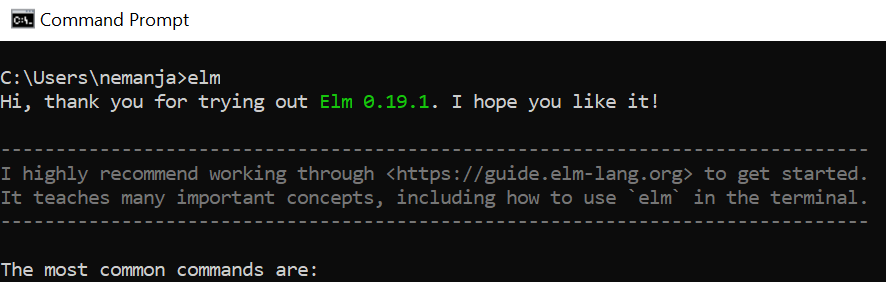
\includegraphics[width=0.95\textwidth]{elm-cmd.png}
  \caption{Elm - Cmd}
\end{figure}

Takođe, mooguća je instalacija pomoću \textbf{npm}
\footnote{Node Package Manager - JavaScript menadžer paketa} alata \cite{npm}.

\section{Osnovne odlike}
Pored \emph{No Runtime Exceptions}, jedna od glavnih odlika ovog jezika jeste
kompilator, koji je izuzetno ugodan za rad. Mnogi programeri smatraju da Elm
kompilator proizvodi najbolje poruke o greškama. Za razliku od drugih, Elm
kompilator objašnjava zašto je došlo do greške i daje predloge za njihovo rešavanje,
a takođe nema kaskadnih poruka. Kreator se vodio razmišljanjem da kompilator treba
da bude asistent, ne samo alat.

Elm koristi svoju verziju \emph{virtualnog DOM-a}, koncepta koji se koristi u mnogim
frontend okruženima. Ideja je da se u memoriji čuva "virtualna" reprezentacija
korisničkog interfejsa  na osnovu koje se ažurira "stvarni" DOM. Još jeda bitna
karakteristika Elm-a je nepromenjivost podataka, što znači da se jednom definisani
podaci ne mogu više menjati. Direkta posldica nepromenjivost podataka je veoma
brzo renderovanje HTML-a, jer se poređenja u virtuelnom DOM-u mogu vršiti po referenci. 
Verzija Elm 0.17 imala je najbrže renderovanje u poređenju sa tadašnjim aktuelnim verzijama 
popularnih okruženja.

Elm se može integrisati i u postojeće JavaScript projetke za implementaciju pojedinačnih komponenti. 
Takođe, moguća je i komunikacija između Elm-a i JavaScripta. 

\section{Elm kao platforma}
Elm sa sobom donosi niz alata (tabela \ref{table:1}) i Elm okruženje (\emph{eng. Elm Runtime}), koji su 
neophodni za razvoj i izvršavanje aplikacija. Elm kod se nalazi u datotekama sa \emph{.elm} ekstenzijom i 
prilikom kompilacije kreira se jedna izlazna \emph{.js} datoteka. U izlaznoj datoteci se pored prevedenog 
koda iz ulaznih \emph{.elm} datoteka nalaze i (runtime) funkcije iz Elm okruženja potrebne za izvršavanje programa.


\begin{table}[h!]
\centering
\begin{tabular}{|l l|} 
 \hline 
 Alati & Kratat opis  \\ [0.5ex] 
 \hline
  \textbf{repl} & Pokretanje interaktivne sesije (\emph{eng. Read-Eval-Print-Loop}) \\ 
  \textbf{init} & Inicijalizacija projekta \\
  \textbf{reactor} & Pokretanje lokalnog servera \\
  \textbf{make} & Upotreba kompilatora \\
  \textbf{install}  & Preuzimanje paketa \\ 
  \textbf{diff} & Prikazivanje razlika između različitih verzija istog paketa \\
  \textbf{bump} & Određivanje broja naredne verzije paketa  \\
  \textbf{publish} & Publikacija paketa \\[1ex] 
 \hline
\end{tabular}
\caption{Elm alati komandne linije}
\label{table:1}
\end{table}

 
Kao zaseban jezik Elm ima i zaseban sistem za upravljanje paketima.
Pokretanjem komande \textbf{elm init} kreira se prazan \emph{src} direktorijum i 
datoteka \emph{elm.json}, u kojoj se pored informacije o tipu projekta (aplikacija ili paket), 
Elm verzije i liste direktorijuma sa kodom, nalazi i spisak paketa koji se koriste u projektu. 
Dodavanje novog paketa se vrši pomoću komande \textbf{elm install} \emph{naziv-paketa}. 
Svi paketi nalaze se na \url{https://package.elm-lang.org/}, nazivi paketa su oblika \emph{autor/ime-paketa}.

Kompilacija se vrši naredbom \textbf{elm make} \emph{<jedna-ili-više-elm-datoteka>},
ukoliko se ne navede izlazna datoteka pomoću argumenta \emph{-{}-output} generisaće 
se \emph{index.html} datoteka sa prevedenim JavaScript kodom. Ostali argumenti ako i
više informacija o drugim alatima može se videti pomoću naredbe \textbf{elm} \emph{naziv-alata} \textbf{-{}-help}

\section{Elm kao jezik}
\begin{displayquote}
"Rekao bih da je Elm ML sa sintaksom poput Haskell-a. Ako poredimo semantiku, Elm je
dosta  sličniji OCaml-u i SML-u." \emph{--Evan Czaplicki \cite{eczaplicki:2015}} 
\end{displayquote}

\textbf{ML} (\emph{eng. Meta Language}) je statički tipiziran programski jezik opšte namene koji je razio 
Robin Miler 1978. godine na Univerzitetu u Edinger. Nastao je pod uticajem LISP-a i ISWIM-a 
(\emph{eng. If you See What I Mean}) jezika, pripada funkcionalnoj i imperativnoj paradigmi. 
Neke od osnovnih karakteristika jesu poklapanje obrazaca, Karijeve funkcije, poziv po vrednosti i posedovanje 
sakupljaca otpadaka. ML nije čist funkcionalan jezik i nema ugrađenu podršku za lenjo izračunavanje. 
U porodicu ML jezika, između ostalih, spadaju i \textbf{Standard ML}, \textbf{OCaml} i \textbf{F{\#}}.


\textbf{Haskell} je čist funkcionalni programski jezik zasnovan na lambda računu.
Naziv je dobio po matematičaru i logičaru Haskelu Bruks Kariju. Haskell je strogo tipiziran, poseduje automatsko 
zaključivanje tipova i lenjo izračunavanje. Jezik je opšte namene, pruža podršku za paralelno i distirbuirano programiranje. 
Haskell omogućava manje grešaka i veću pouzdanost kroz kraći, čistiji i održiviji kod.


\subsection{Osnovni tipovi podataka}
\begin{listing}[ht]
\begin{minted}[bgcolor=black]{haskell}
> 'Z'
'Z' : Char
> "Zdravo!"
"Zdravo!" : String
> True
True : Bool
> 42 / 10 
4.2 : Float
> 42 // 10 --celobrojno deljenje
4 : Int
\end{minted}
\caption{Osnovni tipovi podataka (elm repl)}
\label{listing:tipovi}
\end{listing}

Osnovni tipovi podataka u Elm-u su \textbf{Char}, \textbf{String}, \textbf{Bool}, \textbf{Int} i \textbf{Float}. U Listingu \ref{listing:tipovi} prikazani su osnovni tipovi korišćenjem interpretera, koji nakon unetog izraza ispisuje izračunatu vrednost i tip. 

Tip \textbf{Char} služi za predstavljanje unikod (\emph{eng. unicode}) karaktera. Karakteri se navode između dva apostorfa (\texttt{'a', '0', '\textbackslash t'}...), a moguće je koristiti i unikod zapis  \texttt{'\textbackslash u\{0000\}}' - \texttt{'\textbackslash u\{10FFFF\}'}.

Za razliku od Haskell-a, gde je \textbf{String} zapravo \textbf{Char} lista, u Elm-u je poseban tip i predstavlja sekvencu unikod karaktera. Sekvenca se navodi između jednostrukih ili trostrukih navodnika. 
\begin{listing}[ht]
\begin{minted}[bgcolor=black]{haskell}
> "\t String u jednom redu: escape navodnici \"Zdravo!\""
"\t String u jednom redu: escape navodnici \"Zdravo!\"" : String
>
> """String u više redova
 sa "navodnicima"! """
"String u više redova\n  sa \"navodnicima\"! " : String
\end{minted}
\caption{Stringovi}
\label{listing:string}
\end{listing}

\textbf{Bool} predstavlja logički tip i može imati vrednost \texttt{True} ili \texttt{False}. 

\textbf{Int} se koristi za prikazivanje celih brojeva. Siguran opseg vrednosti je od \(-2^{31}\) do \(2^{31} - 1\), van toga sve zavisi od cilja kopilacije. Kada se prevodi u JavaScript, opseg se proširuje na \(-2^{53}\) do \(2^{53} - 1\) u nekim operacijama, što ne bi važilo ukoliko bi se, nekada kasnije, umesto JavaScript koda generisao WebAssembly, tada bi postojalo prekoračenje celih brojeva(\emph{eng. integer overflow}). Vrednosti se mogu navoditi i u heksadecimalnom obliku  (\texttt{0x2A, -0x2b}).

\textbf{Float} služi za predstavljanje brojeva u pokretnom zarezu po strandardu \emph{IEEE 754}. Vrednosti se mogu navoditi i pomoću eksponencijalnog zapisa, a decimalna tačka se mora nalaziti između dve cifre. Takođe u skup vrednosti spadaju  \texttt{NaN} i \texttt{Infinity}.

U Listingu \ref{listing:brojevi} 
\begin{listing}[ht]
\begin{minted}[bgcolor=black]{haskell}
>0x2A
42 : number
> 1e3
1000 : Float
> 0/0 
NaN : Float
> 1/0 
Infinity : Float
\end{minted}
\caption{Brojevi}
\label{listing:brojevi}
\end{listing}

\subsection{Liste} 



\section{Elm arhitektura}
\chapter{Razvojno okruženje Phoenix i Elixir}

\chapter{Implementacija MSNR portala}

% ------------------------------------------------------------------------------
\chapter{Zaključak}
% ------------------------------------------------------------------------------


% ------------------------------------------------------------------------------
% Literatura
% ------------------------------------------------------------------------------
\literatura

% ==============================================================================

\end{document}